%% LyX 2.1.4 created this file.  For more info, see http://www.lyx.org/.
%% Do not edit unless you really know what you are doing.
\documentclass[12pt,oneside,english]{amsart}
\usepackage{ae,aecompl}
\usepackage[T1]{fontenc}
\usepackage[latin1]{inputenc}
\pagestyle{plain}
\usepackage{amsthm}
\usepackage{amssymb}
\usepackage{graphicx}

\usepackage[paper=letterpaper,left=15mm,right=15mm,top=10cm,bottom=15mm]{geometry}

\makeatletter
%%%%%%%%%%%%%%%%%%%%%%%%%%%%%% Textclass specific LaTeX commands.
\numberwithin{equation}{section}
\numberwithin{figure}{section}

%%%%%%%%%%%%%%%%%%%%%%%%%%%%%% User specified LaTeX commands.
\usepackage{aecompl}
\usepackage{graphicx}
\usepackage{harvard}

\makeatother

\usepackage{babel}
\begin{document}
\begin{center}
Position Auctions
\par\end{center}

One application of auctions which has become increasingly important
over the last few years is their application to online advertizing.
Hallerman\footnote{Hallerman, D (2008) ``US Online Advertizing: Resilient in a Rough
Economy'', \emph{eMarketer, }March.} estimates that online advertizing revenues in the US in 2007 were
at least \$21 billion. \cite{var06} estimates that revenues associated
with the auction of search terms by industry leaders Google and Yahoo
in 2005 were at least \$11 billion. \cite{athell08} provide a less
specific and more conservative estimate of \$10 billion. Either way,
a very large chunk of total advertizing revenue on the internet.

Auctions are used to determine which urls are displayed in the ``Sponsored
Links'' column of the google search page, and the ``Sponsored Results''
column on Yahoo. These auctions are typically referred to as \emph{Position
Auctions. }The technology behind these is remarkable. When a search
word is entered, a page is returned with a set of search results (sometimes
referred to as 'organic links') along with a series of sponsored links.
The primary difference between the two is that the sponsored links
almost always offer to sell you something. The organic links may or
may not involve sales. The sponsored links are useful provided they
contain items the person looking at the page is likely to want to
buy.

The way the urls are made relevant is to associate with each search
term, a set of \emph{positions.}\footnote{It is even more sophisticated than this since Google has quite a bit
of information about the viewer who has entered the search term. When
the viewer sends his search request to Google, his browser passes
a cookie to the google server. The cookie doesn't identify the viewer
directly, but it provides an id that can be used to view a database
that contains information about past searches that have been made
from the same browser. By viewing these, Google can make a good guess
about whether the viewer is male or female, rich or poor, young or
old, etc. The ip adress of the browser can be used to determine where
the viewer is located geographically. Finally, Google knows how likely
it is that the viewer using the current browser will actually follow
a sponsored link. Bids that advertizers submit can be conditioned
on all these things.}\emph{ }The first position is the place at the top right of the page
where the first sponsored link will be placed, the second position
is the second highest link that will be displayed, and so on. Advertizers
who are interested in a particular search term can then bid for that
position in an auction. When you enter your search term, google checks
for bids associated with that search term, then puts the link associated
with the advertizer who submitted the highest bid in the first position\footnote{This isn't quite correct. In fact what they do is to give each advertizer
a score based on how much revenue they expect to earn from that advertizer
given the bid they have submitted. The winner of the auction is the
advertizer whose bid generates the highest expected revenue given
his score. We use the simpler high bid auction to make things a bit
simpler below.}, the second highest bidder in the second highest position, etc, before
sending the page back to you. In other words, every Google page view
results in a new auction being held. In this way, we are all involved
in a large number of auctions.

The payment that a bidder makes depends on the number of viewers who
actually click on the ad. To give some idea of what is involved, Google
estimates that bidders who wan't to have their link displayed in the
third position of the auction associated with the search phrase ``luxury
hotels in London'' would have to pay about \$3.04 per click.

Given the enormous number of times Google and Yahoo are used to conduct
internet searches each day, even a tiny probability of clicking on
a sponsored ad will result in large revenues for the search sites.
Tweaking the design of the auction by modifying reserve prices and
limiting search slots could make a lot of difference to total revenue.
Squeezing revenue is not the only consideration that is important
of course. The search engines also want to attract bidders and viewers
who will click on their ads. We deal with some of these issues later
in the chapter on competition among auctions. This chapter focuses
on the case where the search site faces an exogenous set of advertizers
bidding for positions whose value to them is also exogenous. 


\section{Complete Information}

To begin, we will simply assume that there are $K$ positions which
have associated with them exogenously given values $x_{1}>x_{2}>\cdots>x_{K}>0$.
The idea is that the slot in the first position is the one that consumers
are most likely to click. There are two reasons for this. The first
is simply that it is closest to the cursor which has just clicked
the search box in the top right corner of the browser. A more compelling
argument is a sort of self fullfilling prophecy that we will explain
in more detail later. If consumers think that the most useful ads
are in the first position, then firms will bid more aggressively for
that position. However, the firms that are most likely to win the
auction for that position are the ones who are most likely to make
a sale. So at least when consumers want to buy, their expectation
that the firms from whom they are most likely to buy will be in the
first position are going to be correct. Interpret the $x_{j}$ as
the expected number of clicks at position $j$.

There are $m>K$ firms bidding for the various positions on the web
page. Firm $i$ has characteristic $v_{i}$ that describes its profit
per click. For simplicity, assume that $v_{1}\ge v_{2}\ge\ldots\ge v_{m}$.
The expected revenue of a firm who successfully places their ad in
position $j$ is $v_{i}x_{j}$. Every firm wants the first position,
but not all firms will be willing to pay the same amount for it. All
firms, on the other hand, still earn profits by placing their ads
in lower positions on the web page.

The position auction works as follows: each firm places a bid $b_{i}$.
Lets order the bids so that $b_{1}$ is the highest bid, $b_{2}$
the second highest, and so on.

The first and most desirable position is awarded to the bidder who
submits the highest bid $b_{1}$. He or she then pays the second highest
bid $b_{2}$ for each click. Similarly, the bidder who submits the
$k^{th}$ highest bid wins the $k^{th}$ position, and then pays the
$k+1^{st}$ highest bid for each click he receives. Let the bids be
ordered from highest to lowest. If firm $i$ wins the $k^{th}$ best
position (with a bid $b_{k}$) and pays $b_{k+1}$, then his or her
revenue per click is $\left(v_{i}-b_{k+1}\right)$. Notice that the
firm that wins the $K^{th}$ position (i.e., the lowest or worst position)
pays the highest bid of among bidders who did not win a slot. Given
some array $b_{1},\ldots,b_{m}$ of bids, bidder $i$'s total payoff
when he wins the $k^{th}$ slot is
\[
\left(v_{i}-b_{k+1}\right)x_{k},
\]
 while his payoff is zero if he doesn't win a slot.

As for any problem in which we want to use Nash equilibrium to predict
the outcome, we need to specify the entire game. In other words, we
have to describe the payoff a player earns for any array of bids,
and for any bid that he might submit instead. This is a little complex
here because we have to figure out what will happen when there are
ties. The first complication we have to deal with is that we can't
simply order the bids $b_{1}>b_{2}$ etc, we need to tie a bid to
a bidder. The reason for this complication is that we want to allow
a bidder $i$ to consider submitting bids that are higher than all
the others, higher than all but one of the others, lower than all
the others, etc. The rank of a bidder $i$'s bid is something we are
going to determine as part of our equilibrium.

The strategies of the players are just their bids. So lets make the
switch and imagine that the player whose name is $i$ submits a bid
$b^{i}$. The rank that this bid has depends on the bids of the other
bidders. So lets write the bids submitted by all the players as $b=\left\{ b^{1},\ldots,b^{m}\right\} $.
So lets write $b_{k}\left(b\right)$ to mean the $k^{th}$ highest
bid in the array of bids $b$. For example, $b_{1}\left(b\right)$
is the highest bid submitted by any player, $b_{2}\left(b\right)$
is the second highest bid in the array $b$, and so on. 

We could also write the bids $b$ in a slightly different way. For
example, we could write $b^{-i}$ to mean the array of bids sumitted
by the players other than $i$, then $b_{k}\left(b^{-i}\right)$ represents
the $k^{th}$ highest bid of the bidders \emph{other }than bidder
$i$. Also notice that the vector $\left(b^{i},b^{-i}\right)$ is
the same vector as $b=\left(b^{1},\ldots,b^{i-1},b^{i},\ldots,b^{m}\right)$
except that the elements have been re-ordered. So $b_{k}\left(b\right)=b_{k}\left(b^{i},b^{-i}\right)$.

Now we can write the payoff to each player for every array of bids
in a position auction where the $k^{th}$ position is awarded to the
$k^{th}$ highest bidder who is then charged the $k+1^{st}$ highest
bid for each click. I'll take a shortcut here to make the formula
somewhat simpler.
\begin{equation}
\pi^{i}\left(b^{\prime},b^{-i}\right)=\begin{cases}
\left(v_{i}-b_{1}\left(b^{-i}\right)\right)x_{1} & b^{\prime}>b_{1}\left(b^{-i}\right)\\
\left(v_{i}-b_{k+1}\left(b^{-i}\right)\right)x_{k+1} & \exists k<K:b_{k}\left(b^{-i}\right)>b^{\prime}>b_{k+1}\left(b^{-i}\right)\\
0 & \mbox{otherwise.}
\end{cases}\label{profit-function}
\end{equation}


This is a complicated expression, so well go over it. When a bidder
considers a bid $b^{\prime}$, she first checks the bids of the other
players (i.e., $b^{-i}$) and puts them in order $\left\{ b_{1}\left(b^{-i}\right),\ldots,b_{m}\left(b^{-i}\right)\right\} $.
She then looks to see if her bid $b^{\prime}$ is higher than one
of the $K$ highest bids that the others have submitted. For example,
if there are four bidders (as there will be in the graphical illustration
below), and they submit the bids $\left\{ 2,4,3,6\right\} $ (where
2 is submitted by the bidder with identity 1, 4 by bidder with identity
2, etc, then bidder 3 first takes the other bids $\left\{ 2,4,6\right\} $
and puts them in descending order. This gives her the vector $b_{1}\left(\left\{ 2,4,6\right\} \right)=6$,
$b_{2}\left(\left\{ 2,4,6\right\} \right)=4$ and $b_{3}\left(\left\{ 2,4,6\right\} \right)=2$.
Suppose there are K=3 positions to be won in the auction. She sees
that there is a value for $j$ , i.e., 2, which is less than the number
of positions up for auction, ie, 3, and such that her bid is still
at least as large as $b_{3}\left(\left\{ 2,4,6\right\} \right)=2$
. That means she will win a slot with this bid, that is slot $j+1$
or 3, and pay $b_{3}\left(\left\{ 2,4,6\right\} \right)=2$ for it.
Her profit is then the difference between her value and the price
$2$ multiplied by the average number of clicks associated with slot
3. The math expression above is certainly a more consise way of saying
this. It even works when there are more bidders than slots once you
think it through.

Now you might have noticed already what the shortcut is - I left out
the possibility of equality. The reason I did this (apart from avoiding
writing out a long formula) is that I already know that placing a
bid exactly equal to the bid of another player is a weakly dominated
strategy. It might not matter if the bid doesn't win a slot, but if
it does, then the slot I get would be randomly decided in a lottery
with the bidder with whom I had tied. If I raise the bid ever so slightly,
I would be sure to get the highest of the two slots, which is better.
So I couldn't possibly have an equilibrium is which two bidders submit
the same bid and one of them actually wins a slot.

Now that we have the profit function (\ref{profit-function}), we
basically know the payoffs that each player will get for every array
of bids. That is like knowing what payoffs we put in each cell of
the matrix in a bimatrix game. A Nash equilibrium of this game is
an array of $m$ bids such that no player can improve his payoff given
the bids of the other players. 

We can't really do the gambit thing and check every profile of bids
for profitable deviations. There is a continuum of profiles to worry
about. Solving games like this usually means making a good guess about
what the equilibrium looks like, then trying to verify your guess
is an equilibrium. The educated guess here comes from the observation
that if you win a slot at all, you won't pay what you bid. Instead,
you'll pay what one of the other players bid. So your only real choice
is to decide which slot, if any, you want. The others' bids completely
determine what you pay when you win it.

The second part of the guess comes from the intution that it is likely
to be the case that the bidder with the highest value will want the
best slot, the bidder with the second highest value will want the
second best slot, and so on. Why? Well, at this stage in your reasoning
you can't really articulate why, but is just seems right. Nash equilibrium
is going to give us a conceptual tool that will make it crystal clear
why that intution will work.

WIth that start, lets just guess that each slot with have a price,
say $p_{1}\ge p_{2}\ldots\ge p_{K}$, and that the bidder with the
highest value will have to win the best slot, and so on as we described
above. Since bidders are really only choosing which slot to win, this
will only work if the set of prices satisfies 
\begin{equation}
v_{i}-p_{i}\ge0\label{non-negative}
\end{equation}
 for $i=1,\ldots,K$ and $v_{i}-p_{K}\le0$ for all $i>K$. If this
weren't true, then some of the winners would be sorry to have won.

Also, since players can also win other players' slots by outbidding
them (and they don't have to worry about their actual bid), then for
$K\ge i\ge1$, player $i$ would prefer to win slot $i$ at price
$p_{i}$, than to win any other slot ,
\begin{equation}
\left(v_{i}-p_{i}\right)x_{i}\ge\left(v_{i}-p_{j}\right)x_{j}\label{modular}
\end{equation}
for each $i$ and $j$. 

If we could find a solution to these inequalities, then we could just
have each bidder submit the corresponding bid, i.e., the bidder with
the highest value could submit the bid $v_{1}$, etc. No bidder would
want to outbid any other bidder, because that would violate (\ref{modular}).
This would constitute a Nash equilibrium. Finding a solution to a
set of inequalities -- now we are back in algorithm mode.

To begin, start with the firm with the $K+1^{st}$ highest value,
and suppose that this firm bids its value $v_{K+1}$. This determines
the price of the $K^{th}$ and worst slot to be $v_{K+1}$. If firm
$K$ buys this slot, it earns $\left(v_{K}-v_{K+1}\right)x_{k}\ge0$.
Now for $i<K$, recursively define
\[
\left(v_{i}-p_{i}\right)x_{i}=\left(v_{i}-p_{i+1}\right)x_{i+1}.
\]


A diagram will illustrate why this simple construction will generate
a set of competitive prices. We illustrate for the case where there
are three slots. 

\begin{figure}
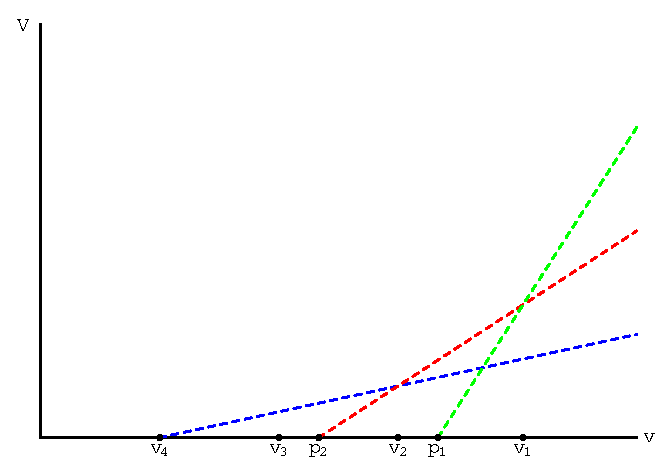
\includegraphics{position_fig1}

\caption{Recursive Construction of Slot Prices}
\end{figure}
The horizontal axis in the picture measures the possible values that
firms can have for slots. The values of the top four firms are marked.
The dashed line with the lowest slope (the blue line in the picture)
is the graph of the function
\[
\left(v-v_{4}\right)x_{3}
\]
which describes the payoff to different firm types when they buy slot
3 at price $v_{4}$. It is flat becase the slope of the line is $x_{3}$,
the click through rate of the worst available slot. The advantage
of drawing this is that it makes it possible to see the profits the
higher valued firms would make from this slot as well. Following our
construction, we choose the price $p_{2}$ for slot 2 that makes the
bidder with value $v_{2}$ just indifferent between purchasing slot
2 at price $p_{2},$ and buying slot 3 at price $v_{4}$. The dashed
red line in the picture represents the payoff function $\left(v-p_{2}\right)x_{2}$.
This line is steeper than the line for the third slot because its
slope is equal to the higher click through rate $x_{2}$. Since the
click through rate $x_{2}$ is higher than the click through rate
for slot 3, $p_{2}$ is going to have to be higher than $v_{4}$.
Since the payoff function given by the red line is steeper than the
one associated with the blue line, firm 3 is going to prefer slot
3 to slot 2 when they are priced this way. The green line (the one
with the steepest slope) shows how to construct the price $p_{1}$
for the most valuable slot. 

Now these prices $v_{4}$, $p_{2}$ and $p_{1}$ satisfy the inequalities
(\ref{non-negative}) and (\ref{modular}). To se why, look at the
outcome for the bidder with value $v_{3}$. He is supposed to win
slot 3 at price $v_{4}$, so the profit he gets from that can be read
as the distance up to the blue dashed line. Similarly he could try
the other slots by paying $p_{2}$ or $p_{1}$, and you can read the
consquences of these choices by measing the distance up to the red
and green lines - at value $v_{3}$, up is down to those lines, which
means that bidder 3 would lose money on these other slots.

On the other hand, bidder 2 is supposed to win slot 2 at price $p_{2}$.
His profit is the distance up to the red line above $v_{2}$. He could
win the lower slot at price $v_{4}$, but if he did, he would get
the same profit because of the way we chose $p_{2}$. Again, if he
tried to win the higher slot, his profit would be negative, which
you can see by reading from the graph.

So the bids, $v_{4}$, $p_{2}$, $p_{1}$ and $v_{1}$ will support
the slot prices that satisfy (\ref{non-negative}) and (\ref{modular}). 

It isn't hard to understand why the firms do this in this example.
They never expect to have to pay what they bid, so there is no reason
for them to worry about their bid, beyond the fact that it secures
the slot they want. Firm 3, for example, knows in this equilibrium
that he will only have to pay $v_{4}$ for the slot.

Second, observe that we can support many Nash equilibria this way.
All we need to do is to make sure that each of the top three firms
makes a profit on the slot they win, and that each prefers their slot
to any other slot. In the picture, just slide the red line to the
left to any position in which firm 3 prefers slot 3 to slot 2 (which
just means the blue line has to be higher than the red line at $v_{3}$).
Similarly, slide the green line to the left lowering $p_{1}$ to any
position at which the blue line is higher than the green line at $v_{2}$.
These changes will generate new Nash equilibrium with new prices for
the different slots. These prices will be lower for slots 1 and 2.

On the other hand, we could go the other way and raise revenues that
are generated by the position auction. We can't just raise bidder
3's bid this time, because if we do, bidder 2 will switch and want
to bid on the worst slot instead of on the second best slot. We could
raise revenues by increasing the bid by bidder 4 however. This may
be one reason that google doesn't explain exactly how they set their
prices. The Nash equilibrium leaves some money on the table for them
if they can set the price of the lowest slot to the value of the third
highest bidder.

A second price auction of the kind we are studying here often has
the feature that bidders will bid their 'valuations'. This won't necessarily
support on equilibrium here as Figure \ref{fig-2} illustrates.

\begin{figure}
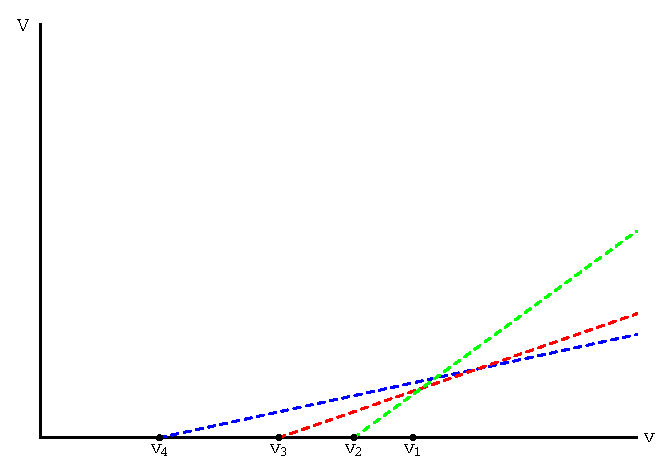
\includegraphics{position_fig2}

\caption{Bidding Values?}
\label{fig-2}
\end{figure}
In this Figure, each bidder bids his own value, which would give prices
$v_{4}$ for slot 3, $v_{3}$ for slot 2 and $v_{2}$ for slot 1.
The it is easy to see from the figure, that at these prices, all three
of the top bidders would prefer to win the third slot. The reason
is that the higher prices that are supported by the bidders values,
aren't warranted given the marginally higher click through rates associated
with the better slots. We have no problem constructing an equilibrium
for this problem, however, it won't support an outcome where bidders
bid their true values.


\subsection*{Exercises}
\begin{enumerate}
\item Can you give an algebraic condition (i.e., and inequality) that will
ensure that there is a Nash equilibrium for this game in which each
bidder bids their value?
\item Using the diagrammatic method, show how to compute prices for the
case where the bidder with the fourth highest value bids $v_{3}$
instead of $v_{4}.$
\item Write down a constrained maximization problem that shows how google
would maximize its ad revenues from this action by setting slot prices
satisfying (\ref{non-negative}) and (\ref{modular}). Can you suggest
an algorithmic method to solve this problem? Could you code it?
\end{enumerate}

\section{Consumer Search}

Apart from the fact that firms bid more than a slot is truly worth
to them in the position auctions, there are a number of characteristics
of this model that seem unrealistic. First, each firm knows exactly
what the values of the other firms are. This is what allows them to
confidently bid way more for a slot than it is worth to them. Perhaps
more important, the click through rates that the firms are bidding
on are unrelated to the characteristics of the firms that are actually
making the bids. Most consumers will only click on sponsored ads if
they feel that these ads will provide them useful information. Whether
they do or not must surely depend on the characteristics they believe
the bidding firms have. Secondly, there is a strong connection between
click through rates and the position of the ad on the web page. Presumably
this reflects the fact that consumers think that ads in a higher slot
are more informative. It would be nice to know exactly why this might
be.

In this section we try to incorporate some of these things into the
analysis. Lets assume first that consumers bear costs when they click
on a sponsored link. There are two reasons this is a reasonable assumption.
First, consumers interest in following a commercial link differ. Some
consumers have a direct an immediate need, while others may be viewing
search results for other reasons. A consumer whose primary interest
is to locate a fact may find it very costly to follow a sponsored
link that may or may not lead him to something that he can buy. Secondly,
even consumers with immediate needs may find sponsored links costly.
The link itself probably won't directly provide the price and product
information they want, causing them to have to search a specific website
while they may be able to find the information they want more effectively
by searching organic links.

Suppose the search cost for consumer $i$ is $s_{i}$ drawn using
a uniform distribution on $\left[0,1\right]$. Lets makes things simple
and assume that there are only two consumers like this. Firms, on
the other hand, are distinguished by the probability with which they
will be able to supply the good the consumers are looking for. Let
$q_{j}$ be the probability with which firm $j$ can supply a consumer.
Again, we'll assume this is drawn using a uniform distribution on
$\left[0,1\right]$. We'll also assume that there are 3 firms competing
for two slots. 

Consumers have value 1 if the link that they click leads a product
they want. The firm at that link also receives revenue 1 in this case.
So the way the auction works is that consumers open a page with 2
sponsored links. A consumer has cost $s_{i}$ of clicking a sponsored
link and discovering whether or not the good that is advertized is
one that they want. Depending on the cost of clicking on the link,
the consumer decides whether or not to click. If the cost is low enough
that the consumer does want to click, we assume that she clicks the
top link first and explain why it makes sense for her to do this in
a bit. If she decides it isn't worth it to follow the sponsored link,
she leaves with zero payoff.

If the firm behind the link has quality $q_{j}$, then a transaction
happens with probability $q_{j}$. In that event the consumers payoff
is $1-s_{i}$ and the firms payoff is $1-b_{i}$ where $b_{i}$ is
the amount that the firm agreed to pay for its advertizing slot when
it won it at auction. If the transaction doesn't happen, the firm
gets nothing from the transaction, but still pays $b_{i}$ for the
click. The consumer then decides again based on her cost, whether
or not to click on the second sponsored link. If she doesn't click,
then she simply leaves the auction having born the search costs associated
with her first click. If she does decide to continue searching, she
meets a firm with whom she transacts with whatever probability $q$
characterizes that firms quality. If no transaction occurs in this
case, she leaves the auction site with payoff equal to minus twice
her search cost.

This model (which is based on \cite{athell08}is relatively simple,
but captures a number of interesting features. First, the value of
the different slot positions to firms is endogenous since the click
through rate will depend on how many consumers have search costs low
enough to induce them to follow the link. The identity of these consumers
is also enogenous since whether or not they want to follow a link
will depend on how likely it is the link will provide them a transaction.
If the firms who are most likely to be able to supply consumers (that
is, firms with high $q$) think that consumers are clicking the top
ad first, then they will be willing to bid more for the first slot.
If they do, then consumers will be quite rational in thinking that
they are more likely to find a transaction if they click the first
link than if they click the second.

This model also resolves one of the issues associated with the position
auction we discussed in the first part of this chapter, since firms
won't know exactly the values of their competitors. This helps make
bidding strategies of the firms more reasonable.

As before, we assume the firms submit bids to the position auction.
He highest bidder is awarded the top slot on the page, and required
to pay the bid of the second highest bidder. Similarly, the second
highest bidder is given the second slot and required to pay the bid
of the third highest bidder.


\subsection{Equilibrium}

To see how the equilibrium unfolds, lets suppose for the moment, that
each firm uses the same bidding strategy $b\left(q\right)$ that is
monotonically increasing in $q$. If the realized qualities of the
three firms are $q_{1}>q_{2}>q_{3}$, then $b_{1}>b_{2}>b_{3}$ and
firm 1 will win the first slot on the page, while firm 3 won't win
any slot at all. From consumers' perpective, the expected quality
of the firm whose advertizement appears in the first slot is the expected
value of the highest of the three qualities of firms who are bidding,
while the expected quality of the firm in the second slot is the expectation
of the second highest quality. As these qualities are uniformly distributed,
it isn't so hard to figure out what these are. For example, there
are three firms who qualify as candidates for the highest quality
firm. Each quality in the interval $\left[0,1\right]$ is equally
likely. For any particular quality $q$ and firm, the probability
that the other two firms have lower qualities is $q^{2}$. So the
expected value of the highest quality firm is
\[
\int_{0}^{1}q\left(3q^{2}\right)dq=\frac{3}{4}.
\]
Similarly, the expected quality of the firm who wins the second slot
can be calculated from the following observation: if this firm has
quality $q$, then the probability that one of the others has lower
quality, while the other has higher quality is $q\left(1-q\right)$.
There other two can be ordered in two different ways, and there are
three different firms who could have the second highest quality. So
the expected quality of the firm in the second slot is
\[
\int q6q\left(1-q\right)dq=\frac{1}{2}.
\]
This begins to explain why it makes sense for consumers to click on
the top ad, since the probability with which they will find what they
are looking for if they click there is $\frac{3}{4}$, while if they
click on the second ad it is only $\frac{1}{2}$. So we will assume
from now on that consumers whose search costs are low enough that
they will want to click on some ad, will choose the top url first.

Their search problem doesn't end at this point, because there is still
a ex ante probability of $\frac{1}{4}$ that they won't find what
they want after clicking on the first ad. The first ad represents
their best chance of finding a useful product. So if they don't find
what they want, then it is bad news, and they should revise their
estimate of the expected quality of the firm at the second position
downward.

To do this, we need to calculate the probability that the consumer
will trade if he clicks on the second link conditional on failing
to trade after clicking on the first link. The easiest way to do this
computation is directly using the distribution of the second order
statistic of firm qualities. If the firm with the second highest quality
has quality $x$, then the expected quality of the firm with the highest
quality is $x+\frac{1-x}{2}$. Conditional on the second best firm's
quality, the probability that the consumer trades with the second
best firm and fails with the first is $x\left(1-x-\frac{1-x}{2}\right)$.
Integrating this across the possible qualities of the second best
firm using the density of the second best firm's quality that we derived
above, then dividing by the probability $\frac{1}{4}$ with which
the consumer fails to trade with the best firm (since we want the
trading probability conditional on failure on the first try), we derive
the probability with which the consumer trades with the second best
firm after failing to find what she want with the first to be $\frac{2}{5}$.
Notice that this is much lower than the expected quality of the second
best firm at the beginning of the search process. Once again, this
is because the failure to trade with the first firm suggests that
the best firm has a relatively low quality. This makes the consumer
more pessimistic about the quality of the firm available at the second
link.

Now we know exactly how the consumer is going to conduct her search.
She perceives a cost of $s_{i}$ of clicking on any link, so she simply
compares the expected quality available by clicking on the link with
her cost. Consumers whose costs exceed $\frac{3}{4}$ won't bother
to click on the sponored links at all. If their costs are below $\frac{3}{4}$,
they will click on the first sponsored link on the page. Some consumers
who do this will find just what they want, and will leave the search
process. 

Those who fail to find what they want after the first link, become
much more pessimistic as we explained. If their costs are between
$\frac{2}{5}$ and $\frac{3}{4}$ they won't bother to click on another
sponsored link. However, those whose costs are below $\frac{2}{5}$
will continue their search and click on the second link.

This is exactly the information needed to determine how valuable the
different slots are to firms. There are two consumers. No matter what
the firm bids, two consumers will click on the first slot with probability
$\left(\frac{3}{4}\right)^{2}$ (which is the proability that both
consumers have search costs below $\frac{3}{4}$). The probability
that only one consumer clicks is $2\left(\frac{3}{4}\right)\left(\frac{1}{4}\right)$,
while the probability there are no clicks at all is $\left(\frac{1}{4}\right)^{2}$.
The revenue that a firm of type $q$ gets from slot 1 is then 
\[
R_{1}\left(q\right)=\left(\frac{3}{4}\right)^{2}2q+2\left(\frac{3}{4}\right)\left(\frac{1}{4}\right)q=\frac{6}{4}q.
\]
On the other hand, a sale through the second slot requires two things
to occur. First, consumers must be unsatisfied at the first link.
Then, in addition, their search costs have to be low enough to induce
them to click on the second link. 

The probability that consumers who want to search fail to transact
after clicking on the first link depends on the quality of the firm
who wins the first link. This characteristic of the position auction
makes it unusual. What it takes to win the top slot depends on what
the firm who wins the second slot bids. So the \emph{revenue }earned
by the firm in the second position depends on its bid. Exactly how
it depends is determined by the equilibrium bidding rule.

To see how, let $b\left(q\right)$ be some monotonic bidding rule
that firms are using to submit bids in the position auction. If a
firm bids $b^{\prime}$, then it wins the first auction if both of
the other firms have qualities such that $b\left(q\right)<b^{\prime}.$
If we write $b^{-1}\left(b^{\prime}\right)$ to be the firm type who
bids $b^{\prime}$, then the probability that the firm wins the first
slot with a bid $b^{\prime}$ is $\left(b^{-1}\left(b^{\prime}\right)\right)^{2}$.
It earns $R_{1}\left(q\right)$ in this event as we explained above.

The probability that it wins the second slot is $2b^{-1}\left(b^{\prime}\right)\left(1-b^{-1}\left(b^{\prime}\right)\right)$.
In this case estimates the expected quality of the firm who won the
best slot to be 
\[
b^{-1}\left(b^{\prime}\right)+\frac{1-b^{-1}\left(b^{\prime}\right)}{2}.
\]
Then the probability that a consumer both has search cost less than
$\frac{2}{5}$ and fails to buy from the firm at the first slot is
$\frac{2}{5}\frac{1-b^{-1}\left(b^{\prime}\right)}{2}$. This gives
the revenue to a firm when it wins the second slot as
\[
R_{2}\left(q,b^{\prime},b\left(\cdot\right)\right)=\left(\frac{1-b^{-1}\left(b^{\prime}\right)}{5}\right)^{2}2q+2\left(\frac{1-b^{-1}\left(b^{\prime}\right)}{5}\right)\left(1-\frac{1-b^{-1}\left(b^{\prime}\right)}{5}\right)q=
\]
\[
2q\left(\frac{1-b^{-1}\left(b^{\prime}\right)}{5}\right).
\]


We can use all this to work out the equilibrium bidding rule. Assuming
the bidding rule is monotonic, the expected payoff of a firm of type
$q$ who bids as if her quality were $q^{\prime}$ is given by 
\[
\left(q^{\prime}\right)^{2}\frac{6}{4}q+2q^{\prime}\left(1-q^{\prime}\right)2q\left[\left(\frac{1-q^{\prime}}{5}\right)\right]-b\left(q^{\prime}\right).
\]
The equilibrium bidding rule should have the property that a firm
of quality $q$ actually wants to bid as if its quality were $q$.
This requires that the derviative of the expression above with respect
to $q^{\prime}$ evaluated at $q$ should be uniformly equal to zero
in $q$. Taking the first derivative in the expression above is a
straightforward but tedious exercise. Since a firm of quality $q$
obviously wants to bid 0, this yields a differential equation whose
solution provides the equilibrium bidding rule.

\bibliographystyle{econometrica}
\bibliography{refer}

\end{document}
